% Formas lineales: el gradiente no es un vector
% Números del texto nuevo verificados con apunte/scripts/cap05_formas_lineales.py
% y apunte/scripts/cap05_transpuesta_normales.py (subsección sec:transpuesta-normales)
\chapter{Formas lineales: el gradiente no es un vector}\label{cap:formas-lineales}

\section{La idea}

El capítulo~\ref{cap:afines} dejó las afinidades como las transformaciones que llevan rectas
paralelas en rectas paralelas; ahora tomamos una familia de rectas paralelas equiespaciadas
como objeto propio. Un vector es una flecha: algo que se suma y se estira. Una \emph{forma
lineal} es una regla que a cada vector le asigna un número, respetando sumas y escalas. En
coordenadas, el vector es una columna, la forma una fila, y la medición es fila contra columna:
\[
  \omega(v)=\begin{pmatrix}\omega_1&\omega_2\end{pmatrix}
  \begin{pmatrix}v_1\\v_2\end{pmatrix}=\omega_1v_1+\omega_2v_2 .
\]
La cota del terreno es el caso que más nos importa. Si en un punto la cota sube \(4\) cm por
cada metro hacia el este y \(3\) cm por cada metro hacia el norte, el cambio de cota para un
desplazamiento \((v_x,v_y)\) es \(0{,}04\,v_x+0{,}03\,v_y\): una forma lineal que \emph{mide}
desplazamientos. Ese diferencial de la cota es lo que el cálculo llama gradiente, y vamos a ver
que se comporta como fila y no como flecha: cuando cambian los ejes, sus componentes cambian al
revés que las de un vector.

\begin{definicion}[Forma lineal]\label{def:forma-lineal}
Una \emph{forma lineal} sobre \(\R^n\) es una función \(\omega\colon\R^n\to\R\) que cumple
\(\omega(u+v)=\omega(u)+\omega(v)\) y \(\omega(\lambda v)=\lambda\,\omega(v)\) para todo par
de vectores \(u,v\) y todo escalar \(\lambda\). Queda determinada por sus valores en los
vectores de una base; en la base canónica se escribe como la fila
\((\omega(e_1),\ldots,\omega(e_n))\).
\end{definicion}

\begin{idea}[Una forma lineal se dibuja como una pila de niveles, no como una flecha]
Los vectores donde \(\omega\) vale \(0,1,2,\ldots\) forman rectas paralelas equiespaciadas
(en \(\R^3\), planos). Para medir un desplazamiento \(w\) no hace falta ningún ángulo:
\(\omega(w)\) es la cantidad de marcas que \(w\) cruza, con signo. Una flecha, en cambio, solo
mide si se le agrega un producto interno. La figura~\ref{fig:fl-pila-flecha} pone las dos
imágenes lado a lado.
\end{idea}

\begin{figure}[htbp]
\centering
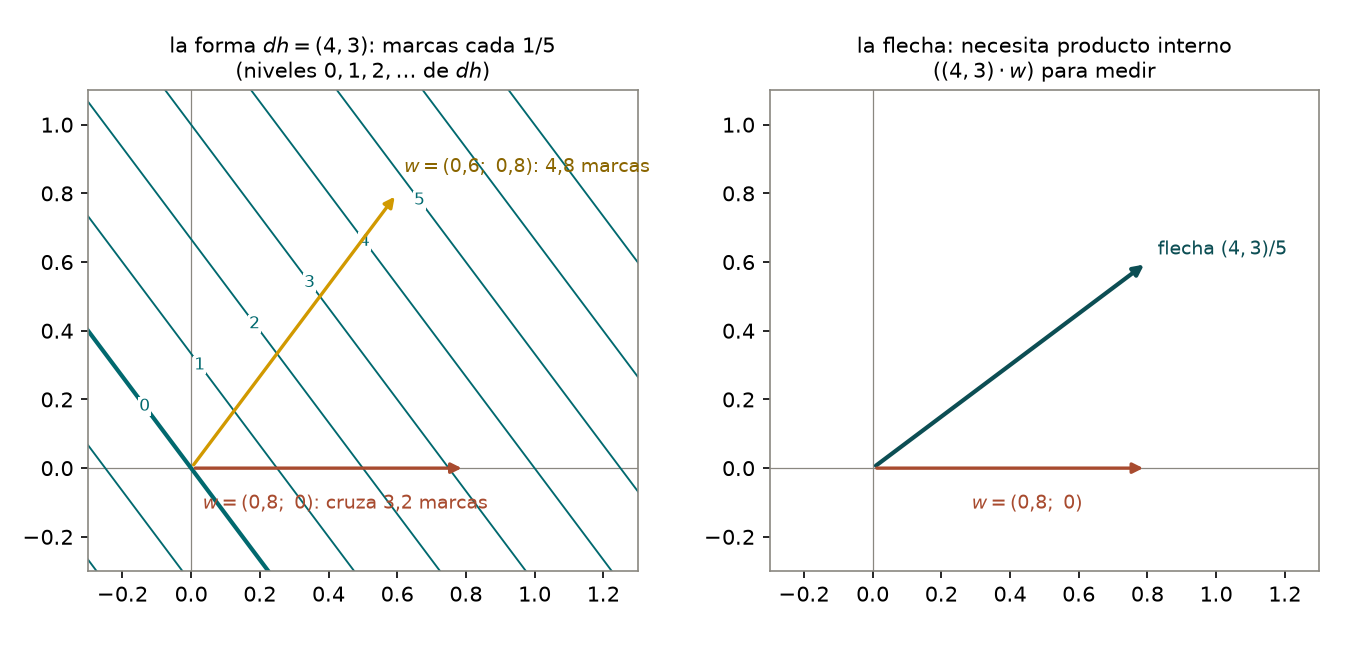
\includegraphics[width=.92\linewidth]{figuras/formas-lineales/fl_pila_vs_flecha.png}
\caption{Izquierda: la forma \(dh=(4,3)\) del ejemplo~\ref{ej:fl-gradiente} como pila de
rectas de nivel, con marcas cada \(1/\lVert(4,3)\rVert=0{,}2\). El desplazamiento
\(w=(0{,}8;\ 0)\) cruza \(3{,}2\) marcas y \(w=(0{,}6;\ 0{,}8)\) cruza \(4{,}8\): son los
valores \(dh(w)\). Derecha: la flecha \((4,3)\), que solo da esos números a través del
producto escalar \((4,3)\cdot w\).}
\label{fig:fl-pila-flecha}
\end{figure}

\unidadInteractiva{06_formas_lineales}{Formas lineales y dualidad}{Explorá: elegí el caso «escala anisótropa diag(2, 1)» y mové el factor \(k\): las marcas de la regla se separan, la fila pasa a \((2/k,\,1)\) y la fila llevada como si fuera un punto deja de ser perpendicular a las marcas nuevas.}


\section{Construcciones, cuentas y ejemplos}

\subsection{Producto vectorial: unir dos puntos, cortar dos rectas}\label{sec:vectorial}

Queremos una operación que, dados dos puntos \(p,q\), devuelva la recta \(\ell=p\times q\)
que los une. Tiene que cumplir que \(p\) y \(q\) estén en esa recta,
\((p\times q)\cdot p=0\) y \((p\times q)\cdot q=0\), o sea, producir un vector
\emph{ortogonal a sus dos argumentos}. Además, con dos veces el
mismo punto no hay recta que determinar: \(p\times p=0\). Estas exigencias, junto con la
linealidad en cada argumento, \emph{obligan} a que la operación sea, a menos de una constante
(que en homogéneas no importa), el producto vectorial de \(\R^3\):
\[
  p\times q=\begin{pmatrix}p_2q_3-p_3q_2\\ p_3q_1-p_1q_3\\ p_1q_2-p_2q_1\end{pmatrix}.
\]

\begin{resultado}[Las dos propiedades que lo definen]
\textbf{Linealidad} en cada argumento, \((2p)\times q=2\,(p\times q)\) y
\((p+p')\times q=p\times q+p'\times q\), y \textbf{antisimetría}, \(p\times q=-\,q\times p\),
que equivale a \(p\times p=0\) porque el único vector igual a su opuesto es el nulo. Son las
propiedades del \emph{área orientada} de un paralelogramo: duplicar un lado duplica el área,
cambiar el orden de los lados cambia la orientación y dos lados paralelos no encierran área.
Por eso \(\lVert p\times q\rVert\) es el área del paralelogramo de lados \(p,q\).
\end{resultado}

Por simetría de la ecuación de incidencia, la misma operación resuelve el problema dual:
\emph{el punto donde se cortan dos rectas es} \(\ell\times m\). Dos rectas paralelas
\((a,b,c)\) y \((a,b,c')\) dan \(\ell\times m=(c'-c)\,(b,-a,0)^T\): un punto ideal, su
dirección común.

\subsection{Formas lineales: la recta como máquina de medir}\label{sec:formas-lineales}

{\small\vspace{1mm}\linkAnimacion{01_dualidad_gradiente}{Animación: dualidad punto–gradiente}\par}

\paragraph{Primero en \(\R\).} Una forma lineal en la recta es multiplicar por un número,
\(\omega(x)=2x\): una regla graduada cuyas marcas \(0,1,2,3,\ldots\) están equiespaciadas a
distancia \(\tfrac12\). En el plano aparecen direcciones que la regla no mide.

\paragraph{Un ejemplo con números chicos.} Sea \(\omega(x,y)=2x+3y\). Con \(v=(1,0)\) da
\(2\); con \((0,1)\), \(3\); con \((1,1)\), \(5\); con \((3,-2)\), \(0\). Es lineal, y basta
conocerla en los dos vectores de la base para conocerla en todos:
\(\omega(x,y)=x\,\omega(1,0)+y\,\omega(0,1)\).

\paragraph{Hecho geométrico: una regla graduada tirada en el plano.} Los puntos donde
\(\omega\) vale lo mismo forman una recta, \(2x+3y=c\), y al variar \(c\) se obtiene una
familia de rectas paralelas equiespaciadas. La forma lineal \emph{es} esa familia: para
medir un punto, miramos qué recta de la familia pasa por él. La recta \(c=0\) pasa por el
origen y contiene la dirección \((3,-2)\), lo que la forma \enquote{no ve} (su núcleo).
El vector \((2,3)\) es perpendicular a todas las rectas de nivel y apunta hacia donde
\(\omega\) crece.

\begin{center}
\begin{tikzpicture}[scale=.78]
  \begin{scope}
    \clip (-3.2,-3.2) rectangle (4.2,3.2);
    \foreach \c in {-6,-4,-2,0,2,4,6,8}
      \draw[teal,line width=.7pt] (-3.2,{(\c+6.4)/3})--(4.2,{(\c-8.4)/3});
    \draw[teal,line width=1.2pt] (-3.2,{6.4/3})--(4.2,{-8.4/3});
    \draw[axisline] (-3.2,0)--(4.2,0);
    \draw[axisline] (0,-3.2)--(0,3.2);
    \draw[rust,line width=1pt,-{Latex[length=2.4mm]}] (0,0)--(1,1.5)
      node[right,font=\small,labelback] {\((2,3)\)};
    \draw[tealdark,line width=1pt,-{Latex[length=2.4mm]}] (0,0)--(1.5,-1)
      node[below right,font=\small,labelback] {\((3,-2)\): \(\omega=0\)};
    \fill[ink] (1,1) circle (2pt) node[above left,font=\small,labelback] {\((1,1)\): \(\omega=5\)};
  \end{scope}
  \foreach \c/\y in {8/-0.13,6/-0.8,4/-1.47,2/-2.13}
    \node[right,font=\scriptsize,text=teal] at (4.2,\y) {\(c=\c\)};
  \foreach \c/\y in {0/2.13,-2/1.47,-4/0.8,-6/0.13}
    \node[left,font=\scriptsize,text=teal] at (-3.2,\y) {\(c=\c\)};
\end{tikzpicture}
\end{center}

\paragraph{Las selectoras y el espacio de las formas.} Las formas más básicas seleccionan una
coordenada: \(\mathsf{x}(x,y)=x\) y \(\mathsf{y}(x,y)=y\). Cualquier otra es combinación de
ellas: \(\omega=2\,\mathsf{x}+3\,\mathsf{y}\). Las formas lineales forman un espacio
vectorial, el \emph{dual} del plano (definición~\ref{def:base-dual}). En la base canónica una
forma se describe con dos números, igual que un vector, pero la escribimos como \emph{fila}:
\[
  \omega(v)=\begin{pmatrix}2&3\end{pmatrix}\begin{pmatrix}x\\y\end{pmatrix}
  =(2,3)\cdot v .
\]
La fila por la columna es el producto interno con el vector \((2,3)\): la forma se
\enquote{disfraza} de vector gracias al producto interno. En coordenadas homogéneas esto ya se
usó: una recta \(\ell=(a,b,c)\) es una forma lineal, un punto \(p\) es un vector, y
\(\ell\cdot p=0\) es la incidencia de la sección~\ref{sec:interno}.

\paragraph{La matriz como pila de formas.} Una transformación lineal del plano devuelve dos
números por cada vector, y cada uno es una forma lineal. Con
\(A=\left(\begin{smallmatrix}2&3\\1&-1\end{smallmatrix}\right)\),
\(A(1,2)^T=(2\cdot1+3\cdot2,\ 1\cdot1-1\cdot2)^T=(8,-1)^T\): la primera fila mide con la regla \(2x+3y\) y la segunda con la regla \(x-y\): aplicar \(A\)
es leer dos reglas graduadas a la vez. El núcleo de \(A\) es el conjunto de puntos donde las
dos reglas marcan cero: la intersección de las rectas \(2x+3y=0\) y \(x-y=0\), que es solo el
origen porque las rectas se cortan (\(\det A=-5\neq0\)). Si en cambio
\(B=\begin{pmatrix}2&3\\4&6\end{pmatrix}\), las dos filas son la misma regla escalada, sus
rectas de nivel cero coinciden, el núcleo es toda la recta \(2x+3y=0\) y \(\det B=0\): es la
sección~\ref{sec:nucleo} vista desde las filas. Y el método del producto cruz para
autovectores (sección~\ref{sec:autovalores}) busca el vector que todas las reglas de
\(A-\lambda I\) marcan en cero.

\paragraph{Cómo se transforma una forma cuando se transforma el vector.} Sea
\(A=\begin{pmatrix}1&1\\0&2\end{pmatrix}\) y \(v=(1,1)\). Entonces \(Av=(2,2)\) y
\(\omega(Av)=2\cdot2+3\cdot2=10\). ¿Qué regla, aplicada al \(v\) original, da ese mismo
\(10\)? La fila por la matriz:
\[
  (2,3)\,A=\bigl(2\cdot1+3\cdot0,\ 2\cdot1+3\cdot2\bigr)=(2,8),
  \qquad (2,8)\cdot(1,1)=10\ \checkmark
\]
El vector se multiplica por \(A\) a la izquierda (columna); la forma, a la derecha (fila):
\(\omega(Av)=(\omega A)(v)\). Una forma lineal se transforma del lado contrario que un vector.

Para \emph{arrastrar la regla junto con la figura}, o sea, encontrar la forma \(\psi\) cuyas
rectas de nivel son las imágenes por \(A\) de las rectas de nivel de \(\omega\), hay que
deshacer \(A\): \(\psi=\omega A^{-1}\). Con
\(A^{-1}=\left(\begin{smallmatrix}1&-1/2\\0&1/2\end{smallmatrix}\right)\),
\(\psi=(2,3)\,A^{-1}=\bigl(2,\ -1+\tfrac32\bigr)=\bigl(2,\tfrac12\bigr)\). Verificación: el punto \((3,-2)\) está en la recta \(\omega=0\); su imagen es
\(A(3,-2)=(1,-4)\), y \(\psi(1,-4)=2-2=0\): sigue en la recta de nivel cero de la regla
arrastrada. El punto \((3,0)\), con \(\omega=6\), va a \((3,0)\) y \(\psi(3,0)=6\).
Hecho geométrico: las rectas de nivel se deforman con el plano y siguen siendo paralelas
equiespaciadas (es una afinidad), pero cambian su separación y su inclinación; por eso los
coeficientes de la forma cambian \enquote{al revés} que los de los vectores.

\paragraph{El gradiente es una forma lineal.} La derivada de una función en un punto es una
regla de este tipo: su recta de nivel cero es la tangente a la curva de nivel, y que
\enquote{el gradiente es perpendicular a la curva de nivel} es la misma figura de arriba
(sección~\ref{sec:gradiente-forma} y ejemplo~\ref{ej:fl-gradiente}).

\begin{resultado}[Dualidad en pocas palabras]
Vector = columna = flecha; forma = fila = familia de rectas (en \(\R^3\), planos) paralelas
equiespaciadas. Una matriz es una pila de formas (filas: núcleo) o una hilera de vectores
(columnas: imagen). Al transformar con \(A\), los vectores van con \(A\) y las formas con
\(A^{-1}\) (o con \(A\) del otro lado, si se pregunta qué regla mide lo mismo). En homogéneas,
puntos y rectas intercambian roles: la dualidad proyectiva.
\end{resultado}

\subsection{Espacio dual y base dual}\label{sec:base-dual}

\begin{definicion}[Espacio dual y base dual]\label{def:base-dual}
El \emph{espacio dual} \((\R^n)^{*}\) es el conjunto de las formas lineales sobre \(\R^n\).
Dada una base \(b_1,\ldots,b_n\) de \(\R^n\), su \emph{base dual} es la familia de formas
\(e^1,\ldots,e^n\) definida por
\[
  e^i(b_j)=\delta_{ij}=\begin{cases}1&\text{si } i=j,\\ 0&\text{si } i\neq j.\end{cases}
\]
\end{definicion}

La forma \(e^i\) es la que \emph{lee la coordenada \(i\)-ésima} en la base \(b\): si
\(v=c_1b_1+\cdots+c_nb_n\), entonces \(e^i(v)=c_i\). Con la base canónica se recuperan las
selectoras \(\mathsf{x}\) e \(\mathsf{y}\) de la sección~\ref{sec:formas-lineales}. Para
una base cualquiera hay una receta matricial: si \(C\) es la matriz con los \(b_j\) en
columnas, la condición \(e^i(b_j)=\delta_{ij}\) dice que la matriz cuyas filas son las
\(e^i\), multiplicada por \(C\), da la identidad. Las filas de \(C^{-1}\) son la base dual.

Toda forma \(\omega\) se escribe en la base dual con los coeficientes
\(\omega_j=\omega(b_j)\): \(\omega=\omega_1e^1+\cdots+\omega_ne^n\). Los coeficientes de un
vector se obtienen \emph{resolviendo} un sistema (\(c=C^{-1}v\)); los de una forma, en
cambio, \emph{evaluando} (\(\omega_j=\omega(b_j)\): la fila \(\omega C\)). La medición se
conserva: \(\omega(v)=\sum_j\omega_jc_j\), porque \((\omega C)(C^{-1}v)=\omega v\).

\begin{ejemplo}[Base dual de una base oblicua]\label{ej:fl-base-dual}
Sea la base \(b_1=(2,0)\), \(b_2=(1,1)\), que no es ortogonal. Con
\[
  C=\begin{pmatrix}2&1\\0&1\end{pmatrix},\qquad
  C^{-1}=\begin{pmatrix}\tfrac12&-\tfrac12\\0&1\end{pmatrix},
\]
la base dual es \(e^1=(\tfrac12,-\tfrac12)\), \(e^2=(0,1)\). Se verifica a mano:
\(e^1(b_1)=1\), \(e^1(b_2)=\tfrac12-\tfrac12=0\), \(e^2(b_1)=0\), \(e^2(b_2)=1\).

Hecho geométrico: las rectas de nivel de \(e^1\) son paralelas a \(b_2\) (la forma no ve a
\(b_2\)) y están espaciadas de modo que \(b_1\) avanza una marca; las de \(e^2\) son
paralelas a \(b_1\). Que \(e^2=(0,1)\) coincida con la selectora \(\mathsf{y}\) se debe a
que \(b_1\) es horizontal y \(b_2\) tiene segunda componente \(1\). En cambio
\(e^1=(\tfrac12,-\tfrac12)\) no es \(\tfrac12\,\mathsf{x}\): si se cambia \(b_2\), cambia \(e^1\)
aunque \(b_1\) siga igual. La forma que lee la primera coordenada depende de toda la base
(figura~\ref{fig:fl-base-oblicua}).

El vector \(v=(3,2)\) tiene coordenadas \(c=C^{-1}v=(0{,}5;\ 2)\): \(v=0{,}5\,b_1+2\,b_2\).
La forma \(\omega=(2,3)\) tiene en la base dual los coeficientes
\(\bigl(\omega(b_1),\omega(b_2)\bigr)=(4,5)\). La medición da lo mismo por los dos caminos:
\(\omega(v)=2\cdot3+3\cdot2=12\) y \(4\cdot0{,}5+5\cdot2=12\).
\end{ejemplo}

\begin{figure}[htbp]
\centering
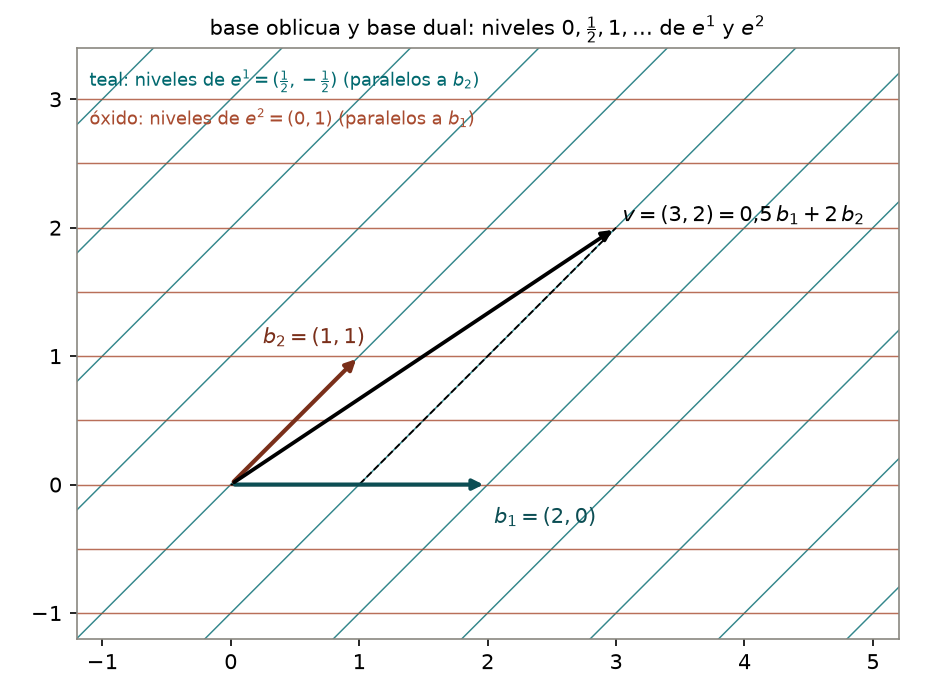
\includegraphics[width=.72\linewidth]{figuras/formas-lineales/fl_base_oblicua.png}
\caption{La base oblicua \(b_1=(2,0)\), \(b_2=(1,1)\) del ejemplo~\ref{ej:fl-base-dual} y las
rectas de nivel \(0,\tfrac12,1,\ldots\) de su base dual: las de \(e^1\) (teal) son paralelas
a \(b_2\); las de \(e^2\) (óxido), paralelas a \(b_1\). Las coordenadas de \(v=(3,2)\) se leen
contando marcas: \(v\) llega a la marca \(0{,}5\) de \(e^1\) y a la marca \(2\) de \(e^2\):
\(v=0{,}5\,b_1+2\,b_2\).}
\label{fig:fl-base-oblicua}
\end{figure}

\subsection{El gradiente como forma lineal}\label{sec:gradiente-forma}

Sea \(h(x,y)\) una función con derivadas parciales continuas, por ejemplo la cota de un
terreno. Para un desplazamiento chico \(v=(v_x,v_y)\) desde un punto \(p_0\),
\[
  h(p_0+v)\approx h(p_0)+\partial_xh(p_0)\,v_x+\partial_yh(p_0)\,v_y .
\]
El término lineal es una forma lineal en \(v\), el \emph{diferencial} de \(h\) en \(p_0\):
\[
  dh_{p_0}(v)=\partial_xh\,v_x+\partial_yh\,v_y
  =\begin{pmatrix}\partial_xh&\partial_yh\end{pmatrix}\begin{pmatrix}v_x\\v_y\end{pmatrix}.
\]
Lo que suele llamarse \enquote{el gradiente} son las componentes de esta fila. Que sea la
mejor aproximación lineal, y cómo se lleva a superficies curvas, es el tema del
capítulo~\ref{cap:derivada}; acá nos interesa como ejemplo de forma.

\begin{ejemplo}[El gradiente de \(h(x,y)=x^2+xy+2y\) en \((1,2)\)]\label{ej:fl-gradiente}
En \(p_0=(1,2)\) vale \(h=7\), \(\partial_xh=2x+y=4\) y \(\partial_yh=x+2=3\), así que
\(dh_{p_0}=(4,3)\). Su acción sobre algunos desplazamientos, comparada con el cambio real
\(h(p_0+w)-h(p_0)\):
\begin{center}
\begin{tabular}{ccc}
desplazamiento \(w\) & \(dh(w)\) & cambio real de \(h\)\\\hline
\((0{,}1;\ 0)\) & \(0{,}4\) & \(0{,}41\)\\
\((0;\ 0{,}1)\) & \(0{,}3\) & \(0{,}3\)\\
\((0{,}08;\ 0{,}06)\) & \(0{,}5\) & \(0{,}5112\)\\
\((0{,}06;\ -0{,}08)\) & \(0\) & \(-0{,}0012\)
\end{tabular}
\end{center}
Los cuatro desplazamientos tienen largo \(0{,}1\). El tercero va en la dirección de \((4,3)\)
y da el máximo, \(0{,}1\cdot5=0{,}5\); el cuarto está en el núcleo de la forma, y \(h\) casi
no cambia: es la dirección de la curva de nivel. Los errores (\(0{,}01\), \(0\),
\(0{,}0112\), \(-0{,}0012\)) son de segundo orden en el largo del desplazamiento.

Hecho geométrico: la recta de nivel cero de la forma afín \(7+dh(p-p_0)\),
\(4(x-1)+3(y-2)=0\), es la tangente en \((1,2)\) a la curva de nivel \(h=7\); las demás
marcas, \(4(x-1)+3(y-2)=c\), son paralelas a ella y están separadas \(1/5=0{,}2\)
(figura~\ref{fig:fl-pila-flecha}).
\end{ejemplo}

\subsection{Cambio de base: la columna y la fila cambian al revés}\label{sec:co-contravariante}

Pasamos de la base canónica a una base nueva \(b_1,\ldots,b_n\), con matriz de cambio de base
\(C\) (los \(b_j\) en columnas). Un mismo desplazamiento tiene coordenadas viejas \(v\) y
nuevas \(v'\); una misma forma, fila vieja \(\omega\) y fila nueva \(\omega'\).

\begin{proposicion}[Componentes contravariantes y covariantes]\label{prop:co-contra}
Con la notación anterior,
\[
  v'=C^{-1}v,\qquad \omega'=\omega C,\qquad \omega'v'=\omega v .
\]
Las componentes del vector cambian con \(C^{-1}\), al revés que la base
(\emph{contravariantes}); las de la forma cambian con \(C\), igual que la base
(\emph{covariantes}). La fila se transforma con la inversa de la matriz que transforma la
columna, y por eso la medición no cambia.
\end{proposicion}

\begin{demostracion}
El vector es \(\sum_jv'_jb_j=Cv'\) y también \(v\), de modo que \(v=Cv'\) y \(v'=C^{-1}v\).
Por la sección~\ref{sec:base-dual}, la componente \(j\)-ésima de la forma en la base dual de
los \(b\) es \(\omega(b_j)\), que es la entrada \(j\) de la fila \(\omega C\). Finalmente
\(\omega'v'=\omega CC^{-1}v=\omega v\).
\end{demostracion}

\begin{ejemplo}[Cambiar la unidad del eje \(x\)]\label{ej:fl-cambio-unidad}
Volvemos a \(dh=(4,3)\) del ejemplo~\ref{ej:fl-gradiente} y medimos \(x\) con una unidad el
doble de larga: \(b_1=(2,0)\), \(b_2=(0,1)\), \(C=\operatorname{diag}(2,1)\). El
desplazamiento \(w=(0{,}1;\ 0)\) pasa a tener coordenadas \(C^{-1}w=(0{,}05;\ 0)\): la
columna se achica. La fila pasa a \(dh\,C=(8,3)\): la componente en \(x\) se duplica, porque
ahora un paso unitario en \(x\) es el doble de largo y \(h\) sube el doble. El producto se
conserva: \(8\cdot0{,}05+3\cdot0=0{,}4\). Con \(w=(0{,}08;\ 0{,}06)\), coordenadas nuevas
\((0{,}04;\ 0{,}06)\), da \(8\cdot0{,}04+3\cdot0{,}06=0{,}5\), igual que antes.

Si, en cambio, tratáramos al gradiente como una flecha y le cambiáramos las componentes como
a un vector, obtendríamos \(C^{-1}(4,3)^T=(2,3)\), y el \enquote{producto} con
\((0{,}05;\ 0)\) daría \(0{,}1\) en lugar de \(0{,}4\): un cambio de cota cuatro veces menor,
solo por haber cambiado la unidad.
\end{ejemplo}

\begin{idea}[El gradiente no es un vector porque sus componentes cambian al revés]
Lo invariante es el número \(dh(w)\), el cambio de cota, que no depende de los ejes
(proposición~\ref{prop:co-contra}): el gradiente es una fila, un elemento del dual.
\end{idea}

\subsection{Cómo se transforman las mediciones}\label{sec:transpuesta-normales}

La proposición~\ref{prop:co-contra} dice cómo cambian las componentes cuando se cambia la
base. Falta la otra mitad: si una transformación \(A\) mueve los puntos, ¿qué les pasa a las
reglas que los miden? La respuesta es la transpuesta, definida sin escribir la matriz.

\begin{definicion}[Transpuesta como adjunta]\label{def:transpuesta-adjunta}
Sea \(A\) una matriz \(n\times n\) y \(\langle\cdot,\cdot\rangle\) el producto interno usual
de \(\R^n\). La \emph{transpuesta} de \(A\), o su \emph{adjunta}, es la única matriz
\(A^T\) tal que
\[
  \langle Au,v\rangle=\langle u,A^Tv\rangle\qquad\text{para todo par }u,v\in\R^n .
\]
Lectura: medir el punto movido \(Au\) con la regla \(\langle\cdot,v\rangle\) da lo mismo que
medir el punto original \(u\) con la regla \(\langle\cdot,A^Tv\rangle\). La transpuesta lleva
la regla \(v\) del lado de llegada a la regla \(A^Tv\) del lado de partida: la que mide a
\(u\) lo mismo que \(v\) mide a \(Au\). No es la regla que viaja junto con los puntos; esa,
la que sigue marcando lo mismo sobre los puntos movidos, es \(A^{-T}v\)
(proposición~\ref{prop:normales-inversa-transpuesta}).
\end{definicion}

\begin{proposicion}[La adjunta existe, es única y es la transpuesta de siempre]\label{prop:transpuesta-propiedades}
\begin{enumerate}[label=(\alph*)]
  \item Hay una sola matriz con la propiedad de la definición~\ref{def:transpuesta-adjunta},
  y su entrada \((i,j)\) es \(A_{ji}\): se obtiene intercambiando filas y columnas de \(A\).
  \item \((AB)^T=B^TA^T\) y, si \(A\) es invertible, \((A^{-1})^T=(A^T)^{-1}\), matriz que se
  escribe \(A^{-T}\).
\end{enumerate}
\end{proposicion}

\begin{demostracion}
(a) Unicidad: si \(B\) y \(C\) cumplen la propiedad, \(\langle u,(B-C)v\rangle=0\) para todo
\(u\); con \(u=(B-C)v\) queda \(\lVert(B-C)v\rVert^2=0\), así que \(Bv=Cv\) para todo \(v\)
y \(B=C\). Entradas: si \(B\) cumple la propiedad, \(B_{ij}=\langle e_i,Be_j\rangle=
\langle Ae_i,e_j\rangle=A_{ji}\). Existencia: con \(B_{ij}=A_{ji}\),
\(\langle Au,v\rangle=\sum_{i,j}A_{ji}u_iv_j=\sum_{i,j}u_iB_{ij}v_j=\langle u,Bv\rangle\).
(b) \(\langle ABu,v\rangle=\langle Bu,A^Tv\rangle=\langle u,B^TA^Tv\rangle\), y por la
unicidad \((AB)^T=B^TA^T\). Con \(B=A^{-1}\): \((A^{-1})^TA^T=(AA^{-1})^T=I^T=I\).
\end{demostracion}

Por ejemplo, con \(A=\left(\begin{smallmatrix}2&1\\0&1\end{smallmatrix}\right)\),
\(u=(1,2)\) y \(v=(3,-1)\): \(Au=(4,2)\) y \(\langle Au,v\rangle=10\);
\(A^Tv=(6,2)\) y \(\langle u,A^Tv\rangle=10\).

\paragraph{Nota terminológica.} En este apunte \enquote{adjunta} se usa solo en el sentido de
la definición~\ref{def:transpuesta-adjunta}. La transpuesta de la matriz de cofactores, que
aparece en la fórmula de la inversa, es otro objeto y se llama \emph{adjugada}
(definición~\ref{def:adjugada}).

\begin{proposicion}[En una rotación, la transpuesta es la inversa]\label{prop:rotacion-transpuesta}
Si \(R\) conserva el producto interno, \(\langle Ru,Rv\rangle=\langle u,v\rangle\) para
todo \(u,v\), entonces \(R^TR=I\) y \(R^T=R^{-1}\). En particular vale para toda rotación
\(R(\theta)\) (proposición~\ref{prop:propiedades-R}).
\end{proposicion}

\begin{demostracion}
Por la definición, \(\langle u,R^TRv\rangle=\langle Ru,Rv\rangle=\langle u,v\rangle\) para
todo \(u\); por el argumento de unicidad de la proposición~\ref{prop:transpuesta-propiedades},
\(R^TRv=v\) para todo \(v\): \(R^TR=I\). Una matriz cuadrada con inversa a izquierda
es invertible con esa misma inversa, así que \(R^T=R^{-1}\). La
proposición~\ref{prop:propiedades-R} dice que \(R(\theta)\) conserva el producto interno.
\end{demostracion}



\begin{proposicion}[Las normales se transforman con la inversa transpuesta]\label{prop:normales-inversa-transpuesta}
Sea \(x'=Ax+c\) una transformación afín con \(A\) invertible y sea \(\ell\) la recta
(hiperplano) \(n\cdot(x-q)=0\). La imagen de \(\ell\) es la recta
\((A^{-T}n)\cdot(x'-q')=0\), con \(q'=Aq+c\): su normal es \(A^{-T}n\), no \(An\). Del mismo
modo, si \(h'(x')=h(x)\), el diferencial cambia como \(dh'=dh\,A^{-1}\), es decir, como
columna, \(dh'^T=A^{-T}dh^T\).
\end{proposicion}

\begin{demostracion}
Si \(p,q\in\ell\), entonces \(n\cdot(p-q)=0\) y la diferencia de las imágenes es
\(Ap+c-(Aq+c)=A(p-q)\). Por la definición~\ref{def:transpuesta-adjunta} aplicada a
\(A^{-1}\) y por la proposición~\ref{prop:transpuesta-propiedades}(b),
\[
  (A^{-T}n)\cdot A(p-q)=n\cdot A^{-1}A(p-q)=n\cdot(p-q)=0 .
\]
Recíprocamente, todo \(x'\) con \((A^{-T}n)\cdot(x'-q')=0\) es imagen de
\(x=A^{-1}(x'-c)\), que cumple \(n\cdot(x-q)=n\cdot A^{-1}(x'-q')=0\). Para el diferencial:
\(h'(x_0'+w')=h(x_0+A^{-1}w')\approx h(x_0)+dh\,A^{-1}w'\), y el término lineal en \(w'\) es
\(dh\,A^{-1}\).
\end{demostracion}

\paragraph{Contraejemplo numérico.} Tomamos la recta por \(q=(1,1)\) con dirección
\(d=(2,1)\) y normal \(n=(-1,2)\) (ecuación \(-x+2y=1\)), y la afinidad
\[
  x'=Ax+c,\qquad A=\begin{pmatrix}2&1\\0&1\end{pmatrix},\quad c=(0{,}5;\ 1),\qquad
  A^{-T}=\begin{pmatrix}0{,}5&0\\-0{,}5&1\end{pmatrix},
\]
que no es ortogonal. La recta imagen pasa por \(q'=Aq+c=(3{,}5;\ 2)\) con dirección
\(d'=Ad=(5,1)\). Si transformamos la normal como un punto, \(An=(0,2)\) y
\((An)\cdot d'=2\neq0\): el ángulo entre \(An\) y la recta imagen es \(78{,}69^\circ\).
Con la inversa transpuesta, \(A^{-T}n=(-0{,}5;\ 2{,}5)\) y \((A^{-T}n)\cdot d'=0\): el ángulo
es \(90^\circ\). La ecuación de la recta imagen es \(-0{,}5\,x'+2{,}5\,y'=3{,}25\); la cumple
también la imagen \((8{,}5;\ 3)\) del segundo punto \(q+d=(3,2)\)
(figura~\ref{fig:fl-normales}).

\begin{figure}[htbp]
\centering
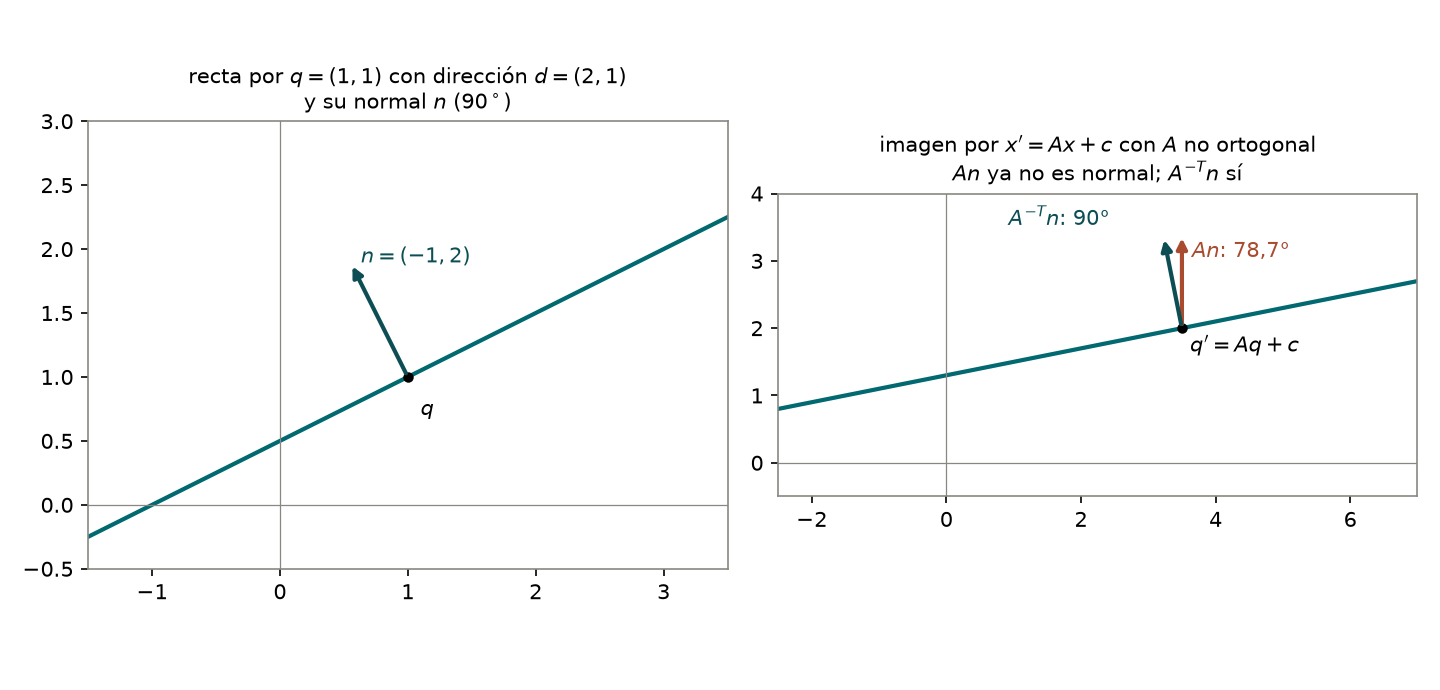
\includegraphics[width=.92\linewidth]{figuras/formas-lineales/fl_normales.png}
\caption{Izquierda: la recta por \(q=(1,1)\) con dirección \((2,1)\) y su normal
\(n=(-1,2)\). Derecha: sus imágenes por \(x'=Ax+c\) con
\(A=\left(\begin{smallmatrix}2&1\\0&1\end{smallmatrix}\right)\). La normal llevada con \(A\)
forma \(78{,}69^\circ\) con la recta imagen; llevada con \(A^{-T}\) sigue siendo perpendicular.}
\label{fig:fl-normales}
\end{figure}

Es la regla de la proposición~\ref{prop:co-contra}: un cambio de coordenadas \(x'=Ax\) es el
cambio de base con \(C=A^{-1}\), y ahí las columnas cambian con \(C^{-1}=A\) mientras que las
filas cambian con \(\omega C=\omega A^{-1}\), que escrito como columna es \(A^{-T}\omega^T\).
Una normal es una fila disfrazada de columna: la forma lineal cuyo núcleo es la dirección de
la recta.

\begin{idea}[Los puntos viajan con \(A\), las reglas con \(A^{-T}\)]
Si la regla \(n\) marcaba cero sobre la recta, la transformada tiene que marcar cero sobre la
recta transformada: hay que deshacer \(A\) antes de medir, y la transpuesta pasa ese \(A^{-1}\)
del lado del punto al de la regla. Solo cuando \(A\) es ortogonal (o ortogonal por un factor
de escala común) \(A^{-T}\) apunta igual que \(A\) y la distinción no se ve.
\end{idea}

\paragraph{Aplicación: la pendiente después de un cambio de coordenadas afín.} Volvemos al
plano del terreno de la sección~\ref{sec:aplicacion-pendiente}, con
\(dh=(a,b)=(0{,}018392;\ 0{,}011622)\) en \((\Delta E,\Delta N)\) en metros. Pasamos a unas
coordenadas locales \(x'=Ax+c\) que giran los ejes \(30^\circ\) y miden el primer eje en
medios metros:
\[
  A=\operatorname{diag}(2,1)\,R(30^\circ)\approx\begin{pmatrix}1{,}732051&-1\\0{,}5&0{,}866025\end{pmatrix},
  \quad c=(100,200),\quad
  A^{-1}\approx\begin{pmatrix}0{,}433013&0{,}5\\-0{,}25&0{,}866025\end{pmatrix},
\]
con \(\det A=2\). Por la proposición~\ref{prop:normales-inversa-transpuesta} la forma en las
coordenadas nuevas es
\[
  dh'=dh\,A^{-1}\approx(0{,}005059;\ 0{,}019261).
\]
El desplazamiento de \(50\) m hacia el acimut \(120^\circ\) de la verificación numérica,
\(W=(43{,}301;\ -25{,}000)\), pasa a \(W'=AW=(100{,}000;\ 0{,}000)\), de \(P_1'=c=(100,200)\)
a \((200,200)\). La cota predicha es la misma en los dos sistemas:
\(dh(W)=dh'(W')\approx0{,}505852\) m, y la cota de llegada es \(32{,}9559\) m en ambos. Si
hubiéramos transformado \(dh\) con \(A\), como un punto, obtendríamos
\((0{,}020234;\ 0{,}019261)\), que aplicado a \(W'\) da \(2{,}023\) m: cuatro veces más.

La dirección de máxima pendiente, en cambio, es una dirección y viaja con \(A\): el versor
\(u\) de acimut \(57{,}71^\circ\) pasa a \(Au\approx(0{,}930045;\ 0{,}885299)\), paralelo a
\(A\,dh^T=(0{,}020234;\ 0{,}019261)\). Es lo que da la
proposición~\ref{prop:vector-asociado} con la métrica de las coordenadas nuevas: el largo
en metros de \(w'\) es \(\lVert A^{-1}w'\rVert\), así que
\(G'=A^{-T}A^{-1}=\operatorname{diag}(0{,}25;\ 1)\) y
\(G'^{-1}dh'^T=AA^TA^{-T}dh^T=A\,dh^T\). La columna \(A^{-T}dh^T=(0{,}005059;\ 0{,}019261)\)
forma \(31{,}70^\circ\) con esa dirección; tomada por error como dirección y llevada de vuelta
al terreno con \(A^{-1}\), apunta al acimut \(37{,}48^\circ\), donde la pendiente es
\(2{,}041\)\,\% y no la máxima, \(2{,}176\)\,\%. La forma se transforma con \(A^{-T}\) y la
dirección de máxima pendiente con \(A\); solo con \(G'=I\) (ejes ortogonales de igual
unidad) coinciden. Los números salen de \texttt{cap05\_transpuesta\_normales.py}.

\section{En profundidad}

\subsection{El producto interno identifica formas con vectores}\label{sec:formas-metrica}

Para convertir una fila en una flecha hace falta un producto interno. Si \(G\) es una matriz
simétrica definida positiva, \(\langle u,v\rangle_G=u^TGv\) es un producto interno (con
\(G=I\), el producto escalar usual), y cada vector \(g\) define la forma
\(\langle g,\cdot\rangle_G\colon v\mapsto g^TGv\).

\begin{proposicion}[El vector asociado a una forma]\label{prop:vector-asociado}
Sea \(G\) simétrica definida positiva y \(\omega\) una forma lineal sobre \(\R^n\) (una fila).
\begin{enumerate}[label=(\alph*)]
  \item Existe un único vector \(g\) tal que \(\omega(v)=\langle g,v\rangle_G\) para todo
  \(v\), y es \(g=G^{-1}\omega^T\).
  \item Entre los vectores de largo \(\lVert u\rVert_G=1\), el que hace máximo a
  \(\omega(u)\) es \(u=g/\lVert g\rVert_G\), y el máximo vale
  \(\lVert g\rVert_G=\sqrt{\omega\,G^{-1}\omega^T}\).
  \item \(g\) es \(G\)-perpendicular a las rectas (hiperplanos) de nivel de \(\omega\), y la
  distancia entre dos niveles consecutivos, medida con \(G\), es \(1/\lVert g\rVert_G\).
\end{enumerate}
\end{proposicion}

\begin{demostracion}
(a) La condición \(g^TGv=\omega v\) para todo \(v\) equivale a \(g^TG=\omega\), o sea
\(Gg=\omega^T\), que tiene solución única porque \(G\) es invertible. (b) Por la desigualdad
de Cauchy--Schwarz para \(\langle\cdot,\cdot\rangle_G\),
\(\omega(u)=\langle g,u\rangle_G\le\lVert g\rVert_G\lVert u\rVert_G=\lVert g\rVert_G\), con
igualdad cuando \(u\) es un múltiplo positivo de \(g\). Además
\(\lVert g\rVert_G^2=g^TGg=\omega G^{-1}GG^{-1}\omega^T=\omega G^{-1}\omega^T\). (c) Si \(v\)
está en el núcleo, \(\langle g,v\rangle_G=\omega(v)=0\). Para pasar del nivel \(0\) al nivel
\(1\) por el camino más corto hay que moverse sobre \(g\): el punto \(tg\) tiene
\(\omega(tg)=t\lVert g\rVert_G^2=1\) con \(t=1/\lVert g\rVert_G^2\), a distancia
\(t\lVert g\rVert_G=1/\lVert g\rVert_G\).
\end{demostracion}

La forma es la misma para cualquier \(G\); el vector asociado no. Con \(G=I\) el disfraz es
transponer, \(g=\omega^T\), y por eso en el plano euclídeo \enquote{el gradiente apunta hacia
donde la función crece más rápido y es perpendicular a las curvas de nivel}. Pero eso es una
afirmación sobre \(g\), y \(g\) depende de con qué se miden largos y ángulos: la métrica es el
único puente entre una regla y una dirección perpendicular (tabla de la
sección~\ref{sec:puntos-formas-grillas}).

\begin{ejemplo}[El mismo gradiente con ejes a \(60^\circ\)]\label{ej:fl-metrica}
Supongamos que las coordenadas \((x,y)\) se miden sobre dos ejes de igual unidad que forman
\(60^\circ\). Los vectores de la base miden \(1\) y su producto interno es
\(\cos60^\circ=\tfrac12\), así que
\(G=\left(\begin{smallmatrix}1&1/2\\1/2&1\end{smallmatrix}\right)\). Tomamos la misma forma \(dh=(4,3)\). El vector asociado es
\(g=G^{-1}(4,3)^T=\bigl(\tfrac{10}3,\tfrac43\bigr)\approx(3{,}333;\ 1{,}333)\), no
\((4,3)\). Comprobamos que mide igual: con \(w=(0{,}1;\ 0)\),
\(g^TGw=0{,}4=dh(w)\); y que es perpendicular (con \(G\)) a la dirección \((3,-4)\) de las
curvas de nivel: \(g^TG(3,-4)^T=0\).

Hecho geométrico (figura~\ref{fig:fl-metrica}): dibujados en el papel con los ejes a
\(60^\circ\), el vector \(g\) forma \(16{,}10^\circ\) con el eje \(x\) y es perpendicular a
las marcas; la columna \((4,3)\) dibujada en esos ejes forma \(25{,}28^\circ\) y no lo es. Las
marcas mismas no cambian: son los puntos donde \(4x+3y\) vale \(0,1,2,\ldots\), sin importar
cómo se dibujen los ejes. Lo que cambia es su separación medida en el papel:
\(1/\sqrt{dh\,G^{-1}dh^T}\approx0{,}240\) en lugar de \(0{,}2\).
\end{ejemplo}

\begin{figure}[htbp]
\centering
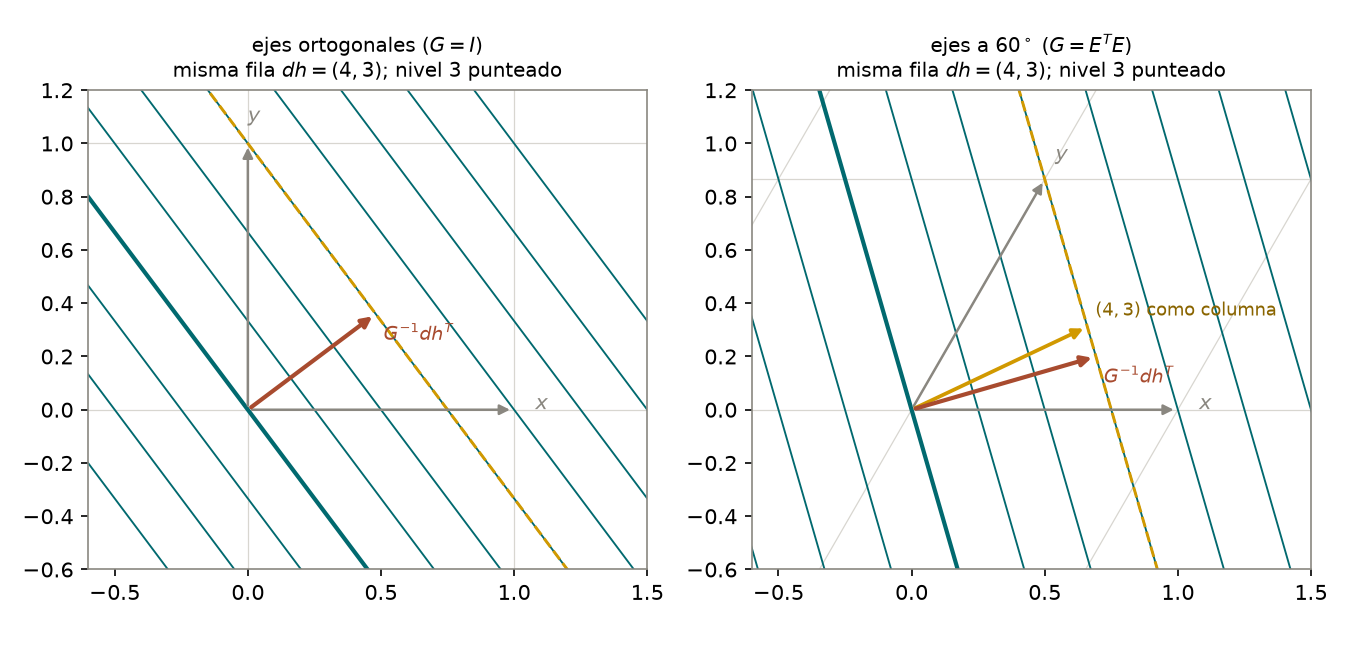
\includegraphics[width=.92\linewidth]{figuras/formas-lineales/fl_metrica.png}
\caption{La fila \(dh=(4,3)\) con ejes ortogonales (izquierda) y con ejes a \(60^\circ\)
(derecha, ejemplo~\ref{ej:fl-metrica}). En los dos paneles las marcas son los puntos donde
\(4x+3y\) es entero, y la punteada es la marca \(3\). La flecha óxido es el vector asociado
\(G^{-1}dh^T\), perpendicular a las marcas en el papel; la dorada es la columna \((4,3)\)
dibujada en los ejes oblicuos, que llega al mismo nivel pero en diagonal.}
\label{fig:fl-metrica}
\end{figure}

\subsection{Curvas de nivel como núcleos de una forma afín}\label{sec:niveles-nucleo}

Cerca de un punto \(p_0\), la función \(h\) se parece a la función afín
\(p\mapsto h(p_0)+dh_{p_0}(p-p_0)\). Sus curvas de nivel, \(h(p_0)+dh_{p_0}(p-p_0)=c\), son
las traslaciones del núcleo de \(dh_{p_0}\) que pasan por los puntos donde la aproximación
vale \(c\). La de \(c=h(p_0)\) es \(p_0+\ker dh_{p_0}\): la recta tangente a la curva de nivel
de \(h\) por \(p_0\). Esta lectura no usa producto interno: la dirección de la curva de nivel
es el núcleo de la forma, y se calcula igual con cualquier unidad y con cualquier par de ejes.

\begin{atencion}[Qué depende de la métrica y qué no]
No dependen de la métrica: el valor \(dh(w)\) sobre un desplazamiento dado, el núcleo
(dirección de la curva de nivel) y qué desplazamientos suben o bajan. Dependen de la
métrica: el vector gradiente \(G^{-1}dh^T\), la dirección de máxima pendiente y el valor
de esa pendiente, porque \enquote{por metro} presupone saber cuánto mide un desplazamiento
(proposición~\ref{prop:vector-asociado}).
\end{atencion}

\subsection{Aplicación topográfica: la pendiente del terreno como forma lineal}\label{sec:aplicacion-pendiente}

En una parcela se nivelaron tres puntos con coordenadas Gauss--Krüger de la faja~5 (el \(5\)
inicial de la coordenada \(E\) indica la faja), en metros:
\begin{center}
\begin{tabular}{lccc}
punto & \(E\) & \(N\) & cota \(h\)\\\hline
\(P_1\) & \(5\,512\,340{,}00\) & \(6\,172\,480{,}00\) & \(32{,}45\)\\
\(P_2\) & \(5\,512\,420{,}00\) & \(6\,172\,510{,}00\) & \(34{,}27\)\\
\(P_3\) & \(5\,512\,360{,}00\) & \(6\,172\,580{,}00\) & \(33{,}98\)
\end{tabular}
\end{center}
En un entorno de unos \(100\) m el terreno se aproxima por un plano. Trabajamos con
diferencias respecto de \(P_1\), porque las siete cifras enteras de las coordenadas absolutas
no aportan nada a la pendiente: \(h=h_0+a\,\Delta E+b\,\Delta N\), con \(h_0=32{,}45\).

\paragraph{El plano.} \(P_2\) y \(P_3\) dan dos ecuaciones:
\[
  \begin{pmatrix}80&30\\20&100\end{pmatrix}\begin{pmatrix}a\\b\end{pmatrix}
  =\begin{pmatrix}1{,}82\\1{,}53\end{pmatrix},
  \qquad a\approx0{,}018392,\quad b\approx0{,}011622 .
\]
Con esos valores el plano reproduce las tres cotas. La forma lineal es
\(dh=(a,b)=(0{,}018392;\ 0{,}011622)\), en metros de cota por metro de desplazamiento:
toma un desplazamiento \((\Delta E,\Delta N)\) y devuelve el cambio de cota.

\paragraph{Pendiente máxima y su acimut.} Con \(E\) y \(N\) en metros los ejes son
ortogonales y de igual unidad, \(G=I\), y por la proposición~\ref{prop:vector-asociado} la
pendiente máxima es \(\sqrt{a^2+b^2}\approx0{,}021756\), o sea \(2{,}176\)\,\% (un ángulo de
\(1{,}246^\circ\) con la horizontal). La dirección es la del vector \((a,b)\); su acimut,
medido desde el norte en sentido horario, es \(\operatorname{atan2}(a,b)\approx57{,}71^\circ\).

\paragraph{Pendiente en una dirección dada.} Para el acimut \(120^\circ\) el versor es
\(u=(\sin120^\circ,\cos120^\circ)\approx(0{,}866;\ -0{,}5)\), y la pendiente en esa
dirección es la acción de la forma sobre el versor,
\(dh(u)=a\cdot0{,}866-b\cdot0{,}5\approx0{,}010117\) (un \(1{,}012\)\,\%), sin necesidad
de conocer el ángulo entre \(u\) y la dirección de máxima pendiente.

\paragraph{Dirección de la curva de nivel.} Es el núcleo de la forma, \(a\,\Delta E+
b\,\Delta N=0\), generado por \((-b,a)\); normalizado,
\((-0{,}534;\ 0{,}845)\), de acimut \(327{,}71^\circ\) (o el opuesto, \(147{,}71^\circ\)).
Difiere en \(90^\circ\) del acimut de máxima pendiente, como corresponde con \(G=I\).

\begin{figure}[htbp]
\centering
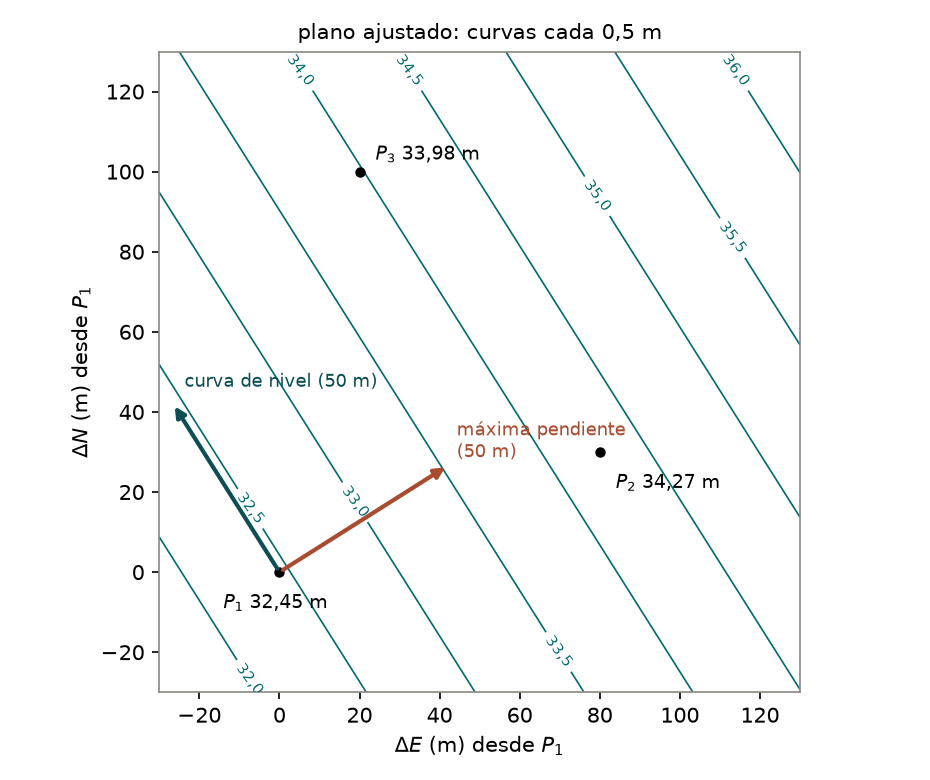
\includegraphics[width=.66\linewidth]{figuras/formas-lineales/fl_terreno.png}
\caption{El plano ajustado a \(P_1,P_2,P_3\): curvas de nivel cada \(0{,}5\) m, que son las
marcas de la forma afín \(32{,}45+a\,\Delta E+b\,\Delta N\). Desde \(P_1\), \(50\) m en la
dirección de máxima pendiente (acimut \(57{,}71^\circ\)) y \(50\) m a lo largo de la curva de
nivel (acimut \(327{,}71^\circ\)).}
\label{fig:fl-terreno}
\end{figure}

\paragraph{Verificación numérica.} Desde \(P_1\):
\begin{center}
\begin{tabular}{lcccc}
dirección & \(\Delta E\) & \(\Delta N\) & \(\Delta h\) & cota\\\hline
máxima pendiente (\(57{,}71^\circ\)) & \(42{,}269\) & \(26{,}709\) & \(1{,}088\) & \(33{,}538\)\\
curva de nivel (\(327{,}71^\circ\)) & \(-26{,}709\) & \(42{,}269\) & \(0{,}000\) & \(32{,}450\)\\
acimut \(120^\circ\) & \(43{,}301\) & \(-25{,}000\) & \(0{,}506\) & \(32{,}956\)
\end{tabular}
\end{center}
Los tres cambios de cota coinciden con \(50\) m por la pendiente correspondiente:
\(50\cdot0{,}021756\approx1{,}088\) m, \(0\) m y \(50\cdot0{,}010117\approx0{,}506\) m.

\paragraph{Si \(N\) estuviera en kilómetros.} Con \(E\) en metros y \(N\) en kilómetros, un
desplazamiento \((\Delta E,\Delta N)\) en metros pasa a tener coordenadas
\((\Delta E,\ \Delta N/1000)\). La forma, por la proposición~\ref{prop:co-contra}, se
multiplica del otro lado: \(dh=(a,\ 1000\,b)\approx(0{,}018392;\ 11{,}6216)\) (\(11{,}62\) m
de cota por kilómetro hacia el norte). Aplicada al desplazamiento de máxima pendiente, ahora
escrito \((42{,}269;\ 0{,}026709)\), da
\(0{,}018392\cdot42{,}269+11{,}6216\cdot0{,}026709\approx1{,}088\) m: el mismo cambio de
cota. La forma no se enteró del cambio de unidades.

La \enquote{flecha gradiente} sí se entera. Si tomamos las componentes
\((0{,}018392;\ 11{,}6216)\) como un desplazamiento en esas coordenadas, sobre el terreno
equivale a \(0{,}018392\) m al este y \(11\,621{,}6\) m al norte: acimut \(0{,}0001^\circ\),
prácticamente el norte, en lugar de \(57{,}71^\circ\). Caminar \(50\) m en esa dirección
cambia la cota en \(50\,b\approx0{,}581\) m, no en \(1{,}088\) m: no es la dirección de
máxima pendiente. El error no está en la forma sino en haberla levantado a vector con
\(G=I\), cuando en las coordenadas \((\text{m},\text{km})\) la métrica es
\(G=\operatorname{diag}(1,10^6)\). Con esa \(G\), \(G^{-1}dh^T=(0{,}018392;\
0{,}0000116)\) en \((\text{m},\text{km})\), que en metros es otra vez \((a,b)\) y apunta a
\(57{,}71^\circ\).

\unidadInteractiva{00_fundamentos}{Fundamentos: puntos, formas lineales y métrica}{Verificá: con el objeto «(b) regla graduada \(w^T\) (el gradiente)» y el caso «estirar Este ×2: diag(2, 1)», comprobá que la fila pasa de \((1,1)\) a \((\tfrac12,1)\), que el mojón conserva su cota y que la perpendicular dibujada en el papel deja de ser la bajada real del terreno.}

\begin{idea}[Aplicación en Inteligencia Artificial: Support Vector Machines (SVM) como formas lineales]
Un \emph{clasificador lineal} separa dos lotes de puntos del plano (dos categorías,
\(y_i=\pm1\)) con una regla \(\omega(x)=w_1x+w_2y+b\): la categoría es el signo de \(\omega\).
Es una forma lineal, una regla graduada tirada sobre la nube: los puntos viven en \(V\), el
clasificador vive en \(V^{*}\), y en coordenadas homogéneas \((x,y,1)\) la traslación \(b\)
entra en la misma fila, \(\omega=(w_1,w_2,b)\), igual que una recta en la
sección~\ref{sec:interno}. La máquina de vectores soporte elige, entre todas las reglas
que separan, la que deja más \emph{margen}: pide \(\omega(x_i)\ge+1\) para una categoría y
\(\le-1\) para la otra, y entre las que cumplen toma la de \(\|w\|\) mínima. Las tres
rectas de nivel \(-1\), \(0\), \(+1\) son el borde de un lado, la frontera y el borde del
otro; los puntos que tocan los bordes son los \emph{vectores soporte}. El ancho de la
franja entre las rectas \(-1\) y \(+1\) es \(2/\|w\|\), porque la separación entre curvas de
nivel consecutivas es \(1/\|w\|\) (proposición~\ref{prop:vector-asociado}), y esa cuenta
necesita el producto interno: sin métrica hay regla, pero no hay ancho. Ejemplo con enteros:
categoría \(+1\) en \((1,1)\) y \((2,0)\),
categoría \(-1\) en \((-1,-1)\) y \((-2,0)\). La frontera de margen máximo es \(x+y=0\) con
\(w=(\tfrac12,\tfrac12)\), \(b=0\): los cuatro puntos dan \(\omega=\pm1\) exacto (los cuatro
son vectores soporte) y el ancho es \(2/\|w\|=2\sqrt2\); la recta vertical \(x=0\) también
separa, pero con ancho \(2\) (verificado con \texttt{scipy.optimize}). La unidad
\texttt{06\_formas\_lineales}
(apéndice~\ref{ap:notebooks}) lo dibuja con el helper \texttt{svm\_margen\_duro\_2d} de
\file{cb104.py}: mové un punto y mirá cómo gira la regla.
\end{idea}

\section{Ejercicios con solución}

\begin{ejercicio}\label{ex:fl-fila}
Una forma lineal \(\omega\) sobre \(\R^2\) cumple \(\omega(1,2)=5\) y \(\omega(3,-1)=1\).
Escribila como fila y hallá la dirección de su núcleo y la separación (euclídea) entre dos
rectas de nivel consecutivas. ¿Cuánto vale \(\omega(4,1)\)?
\end{ejercicio}
\solucion{Con \(\omega=(p,q)\): \(p+2q=5\) y \(3p-q=1\), de donde \(\omega=(1,2)\). El
núcleo es la recta \(x+2y=0\), de dirección \((2,-1)\) (se verifica \(\omega(2,-1)=0\)). La
separación entre niveles es \(1/\lVert(1,2)\rVert=1/\sqrt5\approx0{,}447\). Por linealidad,
\(\omega(4,1)=\omega(1,2)+\omega(3,-1)=6\), igual que \(1\cdot4+2\cdot1\).}

\begin{ejercicio}\label{ex:fl-base-dual}
Hallá la base dual de \(b_1=(1,1)\), \(b_2=(-1,2)\). Escribí \(v=(1,4)\) en la base
\(b\) y \(\omega=(3,1)\) en la base dual, y comprobá que \(\omega(v)\) da lo mismo con las
dos escrituras.
\end{ejercicio}
\solucion{\(C=\left(\begin{smallmatrix}1&-1\\1&2\end{smallmatrix}\right)\), \(\det C=3\),
\(C^{-1}=\frac13\left(\begin{smallmatrix}2&1\\-1&1\end{smallmatrix}\right)\); la base dual
son sus filas: \(e^1=(\tfrac23,\tfrac13)\), \(e^2=(-\tfrac13,\tfrac13)\) (se verifica
\(e^1(b_2)=-\tfrac23+\tfrac23=0\)). Coordenadas de \(v\): \(C^{-1}v=(2,1)\), o sea
\(v=2b_1+b_2\). Coeficientes de \(\omega\): \((\omega(b_1),\omega(b_2))=(4,-1)\). Entonces
\(4\cdot2+(-1)\cdot1=7=3\cdot1+1\cdot4\).}

\begin{ejercicio}\label{ex:fl-cambio-base}
Sea \(h(x,y)=x^2y\) y \(p_0=(1,3)\). (a) Escribí \(dh_{p_0}\) como fila. (b) En la base
\(b_1=(1,0)\), \(b_2=(1,1)\), hallá la fila de \(dh_{p_0}\) y la columna del desplazamiento
\(w=(0{,}2;\ 0{,}1)\), y comprobá que el producto no cambia. (c) ¿Qué se obtendría si se
transformaran las componentes del gradiente como las de un vector?
\end{ejercicio}
\solucion{(a) \(\partial_xh=2xy=6\), \(\partial_yh=x^2=1\): \(dh_{p_0}=(6,1)\), y
\(dh(w)=6\cdot0{,}2+1\cdot0{,}1=1{,}3\) (el cambio real, \(h(1{,}2;\,3{,}1)-h(1,3)\), es
\(1{,}464\)). (b) \(C=\left(\begin{smallmatrix}1&1\\0&1\end{smallmatrix}\right)\); fila
nueva \(dh\,C=(6,7)\), columna nueva \(C^{-1}w=(0{,}1;\ 0{,}1)\), producto
\(0{,}6+0{,}7=1{,}3\). (c) \(C^{-1}(6,1)^T=(5,1)\) y \((5,1)\cdot(0{,}1;\ 0{,}1)=0{,}6\neq1{,}3\):
el resultado dependería de la base, que es lo que una medición no puede hacer.}

\begin{ejercicio}\label{ex:fl-selectora-60}
Con los ejes a \(60^\circ\) del ejemplo~\ref{ej:fl-metrica}, considerá la selectora
\(\mathsf{x}=(1,0)\). Hallá su vector asociado \(g=G^{-1}\mathsf{x}^T\), su largo
\(\lVert g\rVert_G\) y la separación entre las rectas \(x=0\) y \(x=1\). Interpretá: ¿el
\enquote{gradiente de \(x\)} apunta sobre el eje \(x\)?
\end{ejercicio}
\solucion{\(g=G^{-1}(1,0)^T=(\tfrac43,-\tfrac23)\approx(1{,}333;\ -0{,}667)\), con
\(\lVert g\rVert_G=\sqrt{\mathsf{x}\,G^{-1}\mathsf{x}^T}=\sqrt{4/3}\approx1{,}155\). La
separación entre \(x=0\) y \(x=1\) es \(1/1{,}155\approx0{,}866=\sin60^\circ\): las rectas
\(x=\text{cte}\) son paralelas al eje \(y\), y su distancia es la altura del paralelogramo
de lados unitarios a \(60^\circ\). Dibujado en el papel, \(g\) es \((1;\ -0{,}577)\),
perpendicular al eje \(y\) y no paralelo al eje \(x\): la coordenada \(x\) crece más rápido
en dirección perpendicular a sus propias curvas de nivel, que no es la del eje.}

\begin{ejercicio}\label{ex:fl-pendiente-dada}
Un terreno sube con pendiente máxima del \(3\)\,\% en la dirección de acimut \(210^\circ\).
Escribí la forma \(dh=(a,b)\) en \((\Delta E,\Delta N)\) en metros, el cambio de cota al
desplazarse \(40\) m al este y \(40\) m al norte, y la pendiente en la dirección de acimut
\(300^\circ\).
\end{ejercicio}
\solucion{\(dh=0{,}03\,(\sin210^\circ,\cos210^\circ)\approx(-0{,}015;\ -0{,}02598)\).
\(40\) m al este: \(\Delta h=40a=-0{,}600\) m; \(40\) m al norte: \(\Delta h=40b\approx
-1{,}039\) m. El acimut \(300^\circ=210^\circ+90^\circ\) es el de la curva de nivel:
\(dh(\sin300^\circ,\cos300^\circ)=0\), pendiente \(0\)\,\%.}

\begin{ejercicio}\label{ex:fl-normales}
Sea \(A=\left(\begin{smallmatrix}1&2\\0&1\end{smallmatrix}\right)\) y la recta \(x+y=1\), de
normal \(n=(1,1)\) y dirección \(d=(-1,1)\). (a) Calculá \(A^{-T}\) y la ecuación de la
imagen de la recta por \(x'=Ax\); comprobala con las imágenes de \((1,0)\) y \((0,1)\).
(b) ¿Qué ángulo forma \(An\) con la recta imagen? ¿Y \(A^{-T}n\)?
\end{ejercicio}
\solucion{(a) \(A^{-1}=\left(\begin{smallmatrix}1&-2\\0&1\end{smallmatrix}\right)\) y
\(A^{-T}=\left(\begin{smallmatrix}1&0\\-2&1\end{smallmatrix}\right)\), así que
\(A^{-T}n=(1,-1)\). Por la proposición~\ref{prop:normales-inversa-transpuesta}, como
\(n\cdot x=(A^{-T}n)\cdot Ax\), la recta imagen es \(x'-y'=1\). En efecto, \((1,0)\mapsto(1,0)\)
y \((0,1)\mapsto(2,1)\), y los dos cumplen \(x'-y'=1\). (b) La dirección imagen es
\(Ad=(1,1)\). Con \(An=(3,1)\): \((An)\cdot(Ad)=4\neq0\), y el ángulo entre \(An\) y la
recta imagen es \(26{,}57^\circ\), lejos de \(90^\circ\). Con \(A^{-T}n=(1,-1)\):
\((A^{-T}n)\cdot(Ad)=0\), ángulo de \(90^\circ\).}
